\begin{figure*}
  \vspace{-1.0em}
  \centering
  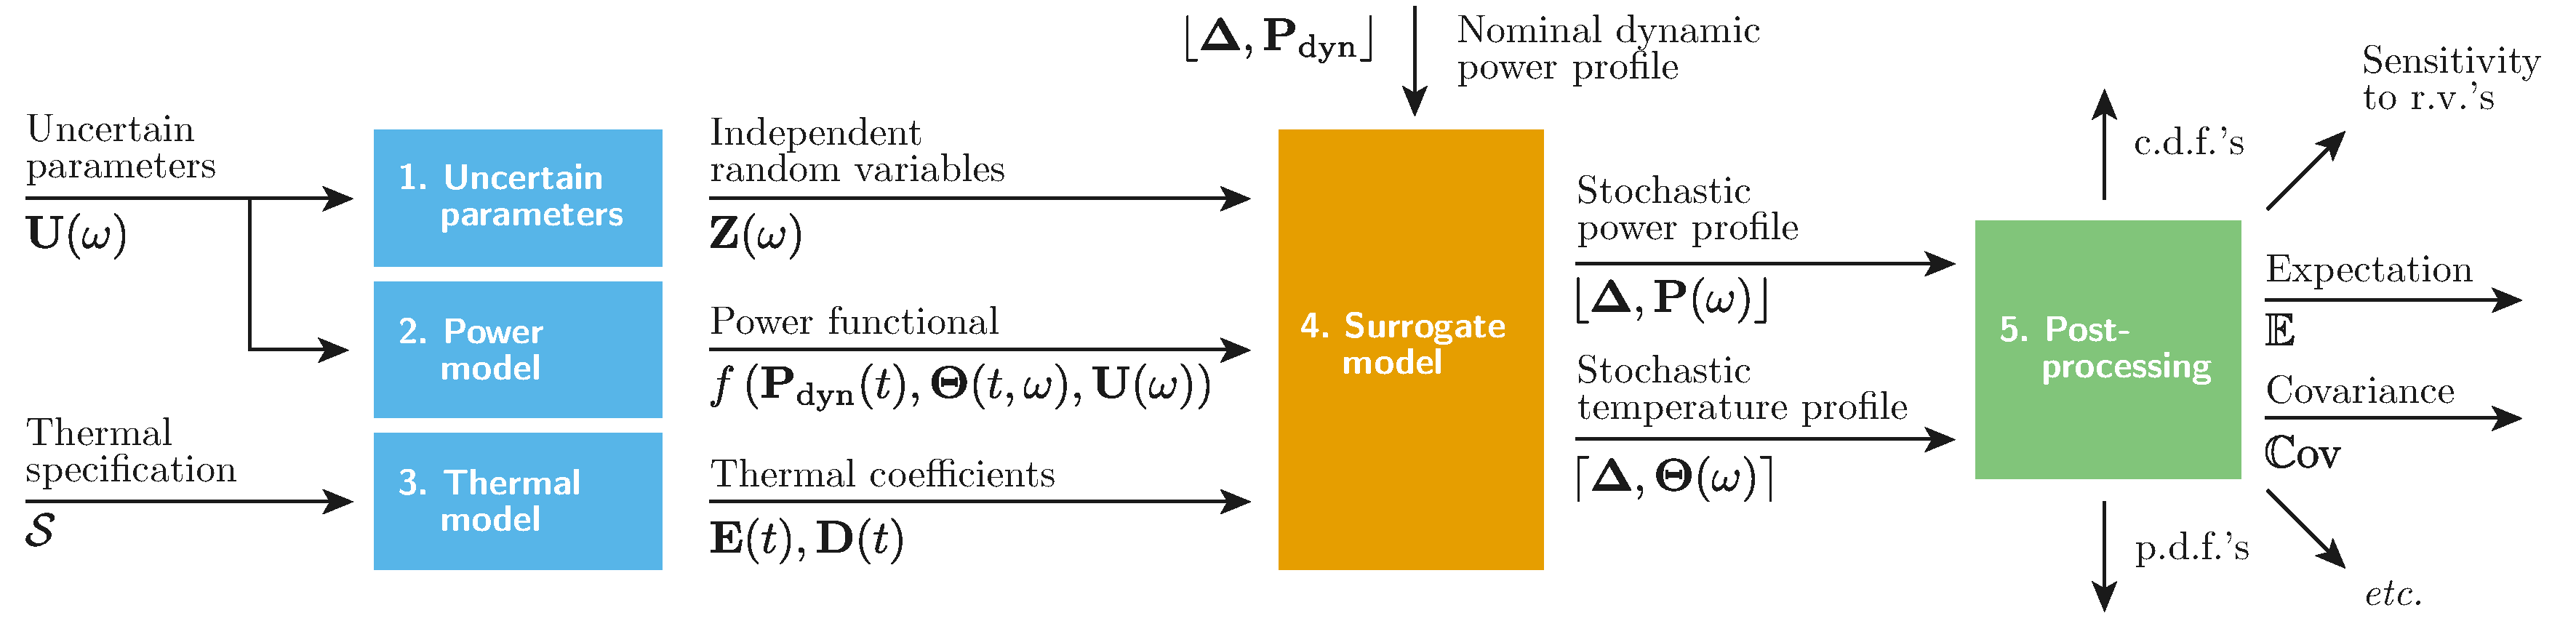
\includegraphics[width=1\textwidth]{include/assets/algorithm.pdf}
  \vspace{-1.0em}
  \caption{The structure of the proposed framework.}
  \flabel{algorithm}
  \vspace{-1.0em}
\end{figure*}

The probability space that we shall reside in is defined as a triple $(\outcomes, \sAlgebra, \pMeasure)$ where $\outcomes$ is a set of outcomes, $\sAlgebra \subseteq 2^\outcomes$ is a $\sigma$-algebra on $\outcomes$, and $\pMeasure: \sAlgebra \to [0, 1]$ is a probability measure \cite{maitre2010}.
Loosely speaking, an $n$-dimensional random variable is then a mapping $\v{X}: \o \in \outcomes \mapsto \v{X}(\o) \in \real^n$.
In what follows, the probability space $(\outcomes, \sAlgebra, \pMeasure)$ is always implied.

Consider a heterogeneous electronic system that consists of $\nprocs$ processing elements and is equipped with a thermal package.
\updated{The processing elements are the active components of the system identified at the system level (ALUs, FPUs, caches, \etc).
Let $\system$ be a thermal specification of the system defined as a collection of temperature-related information: (a) the floorplans of the active layers of the chip; (b) the geometry of the thermal package; and (c) the thermal parameters of the materials that the chip and package are made of (\eg, the silicon thermal conductivity and specific heat).}

A (transient) power profile $\profileP$ is defined as a tuple composed of a data matrix $\mP = (\vP_i) \in \real^{\nprocs \times \nsteps}$, $\vP_i \in \real^\nprocs$, that captures the power dissipation of the $\nprocs$ processing elements at $\nsteps$ moments of time and a (column) vector $\partition{\mP} = (\t_i) \in \real^{\nsteps}$ with positive and strictly increasing components that specifies these moments of time.
The definition of a (transient) temperature profile $\profileT$ is the same as the one for power except that the data matrix $\mTO$ contains temperature.

\updated{The system depends on a set process parameters, which are uncertain at the design stage; these parameters are denoted by a random vector $\vU(\o)$.
Once the fabrication process yields a particular outcome $\o \in \outcomes$, $\vU(\o)$ takes (potentially) different values for each fabricated chip individually and stay unchanged thereafter.
Consequently, $\vU(\o)$ leads to deviations of the actual power dissipation from nominal values and, thus, to deviations of temperature from the one corresponding to the nominal power consumption.}
In what follows, we shall make a distinction between deterministic and stochastic profiles.
In the latter case, the power and temperature profiles are denoted by $\profileP{\o}$ and $\profileT{\o}$, respectively.

\updated{The goal of this work is to develop a system-level probabilistic framework for power-temperature analysis (PTA) of electronic systems where the actual power dissipation and temperature are stochastic due to their dependency on the set of uncertain parameters $\vU(\o)$.}\footnote{\updated{Although the focal point of this paper is process variation, there can be other uncertainties such as those related to the system load and environment.}}
The user is required to: (a) provide a thermal specification of the platform $\system$; (b) have prior knowledge (or belief) on the probability distribution of the uncertain parameters (\sref{uncertain-parameters}); and (c) specify a power model, in which $\vU(\o)$ is an input (\sref{power-model}).
\updated{The framework should provide the user with the tools to analyze the system under a given workload, without imposing any constraints on the nature/origins of this workload, and obtain the corresponding stochastic power $\profileP{\o}$ and temperature $\profileT{\o}$ profiles with a desired level of accuracy and at low costs.}
